\thispagestyle{empty}
\newcommand{\edisi}[1]{%
\DeclareFixedFont{\PT}{T1}{ppl}{b}{}{0.7in}
\DeclareFixedFont{\PTit}{T1}{ppl}{b}{it}{0.7in}
\DeclareFixedFont{\PTsmall}{T1}{ppl}{b}{it}{0.25in}
\DeclareFixedFont{\PTsmaller}{T1}{ppl}{b}{it}{0.175in}
\DeclareFixedFont{\PTsmallest}{T1}{ppl}{b}{it}{0.15in}

\begin{pspicture}(14cm,2cm)
\rput[rb](10.35cm,3cm){\PTsmallest {#1}}
\rput[lb](-0.5cm,1.5cm){\PT {WARTA IMAN}}
\rput[lb](1cm,0.5cm){\PTsmall {Lingkungan St. Petrus Maguwo}}
\end{pspicture}%
}

\newcounter{kgkcounter}[chapter]
\renewcommand{\thekgkcounter}{\arabic{kgkcounter}. }

\NewDocumentCommand\kgk{ s m } {\refstepcounter{kgkcounter}\textbf{\flushleft %
   \IfBooleanTF{#1}{%
	%
   }{% 
   \thekgkcounter%  
   }%
 #2}\\}

\newcommand{\kutipan}[1]{%
\noindent{\framebox{\parbox{10cm}{\centering\emph{#1}}}}}

\makeatletter
\renewcommand{\@makeschapterhead}[1]{%
  {\parindent \z@ \centering \normalfont
    \interlinepenalty\@M \Large \bfseries #1\par\nobreak \vskip 20\p@ }}
\renewcommand{\section}{\@startsection {section}{1}{\z@}%
                                   {-3.5ex \@plus -1ex \@minus -.2ex}%
                                   {1ex \@plus.2ex}%
%                                   {\normalfont\normalsize\bfseries\centering}}
                                   {\normalfont\normalsize\bfseries}}
\renewcommand\subsection{\@startsection{subsection}{2}{\z@}%
                                     {-3.25ex\@plus -1ex \@minus -.2ex}%
                                     {1ex \@plus .2ex}%
                                     {\normalfont\normalsize\bfseries}}
\renewcommand\subsubsection{\@startsection{subsubsection}{3}{\parindent}%
                                    {3.25ex \@plus1ex \@minus.2ex}%
                                    {-1em}%
                                    {\normalfont\normalsize\bfseries}}

\makeatother

\makeatletter  % Allow the use of @ in command names
\long\def\@makecaption#1#2{%
  \vskip\abovecaptionskip
  \sbox\@tempboxa{{#1#2}}%
  \ifdim \wd\@tempboxa >\hsize
    {#1#2\par}
  \else
    \hbox to\hsize{\hfil\box\@tempboxa\hfil}%
  \fi
  \vskip\belowcaptionskip}
\makeatother   % Cancel the effect of \makeatletter

\newcommand{\chap}[1]{%
    \chapter*{#1}
	\addcontentsline{toc}{chapter}{#1}
    }

\newcommand{\sumber}[1]{%    
	\begin{flushright}
	{\emph{#1}}
	\end{flushright}
}
\newcommand{\qti}[1]{%    
	\begin{quote}
	{\emph{#1}}
	\end{quote}
}

\hyphenation{sa-u-da-ra-ku}
\hyphenation{ke-ri-ngat}
\hyphenation{je-ri-tan}
\hyphenation{hu-bung-an}
\hyphenation{me-nya-dari}
\hyphenation{Eng-kau}
\hyphenation{ke-sa-lah-an}
\hyphenation{ba-gai-ma-na}
\hyphenation{Tu-han}
\hyphenation{di-per-ca-ya-kan}
\hyphenation{men-ja-uh-kan}
\hyphenation{bu-kan-lah}
\hyphenation{per-sa-tu-kan-lah}
\hyphenation{ma-khluk}
\hyphenation{Sem-buh-kan-lah}
\hyphenation{ja-lan}
\hyphenation{mem-bu-tuh-kan}
\hyphenation{be-ri-kan-lah}
\hyphenation{me-ra-sa-kan}
\hyphenation{te-man-ilah}
\hyphenation{mem-bi-ngung-kan}
\hyphenation{di-ka-gum-i}
\hyphenation{ta-ngis-an-Mu}
\hyphenation{mi-lik-ilah}

\renewcommand{\figurename}{~}
\renewcommand\thefigure{~}

\setlist{noitemsep}
\renewcommand{\thesection}{\Alph{section}}

\newcommand{\executeiffilenewer}[3]{%
	\ifnum\pdfstrcmp{\pdffilemoddate{#1}}%
	{\pdffilemoddate{#2}}>0%
	{\immediate\write18{#3}}\fi%
	}
\newcommand{\includesvg}[1]{%
	\executeiffilenewer{#1.svg}{#1.pdf}%
	{inkscape -z -D --file=#1.svg %
	--export-pdf=#1.pdf --export-latex}%
	\input{#1.pdf_tex}%
	}
\edisi{Juli 2012}

\vspace{0.5cm}

\begin{center}
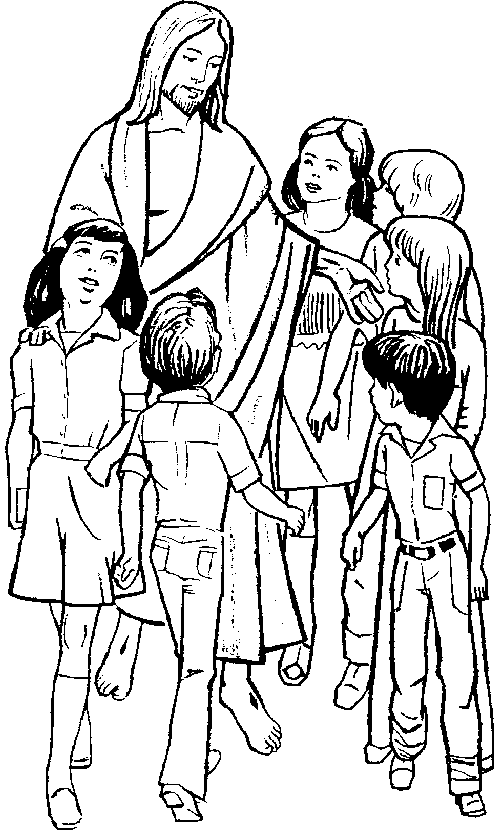
\includegraphics[scale=0.35]{gambar/Xton.png}
\end{center}

\vspace{0.5cm}

\begin{center}
{\PTsmall {Hanya dengan mengetahui jati dirinya sesuai yang dikehendaki Tuhan, maka OMK bisa membangun dunia dan handal}}
\end{center}

\newpage

\begin{parcolumns}[colwidths={1=0.7\textwidth},distance=0.4cm]{2}
\colchunk{
\parbox[t]{0.7\textwidth}{
\newpage

\chapter*{Dari Redaksi}
\footnotesize
\indent{Berkah Dalem,}
Bulan Maret sudah memasuki masa Prapaskah. Tidak ada salahnya jika kita mengambil tema \textit{Prapaskah} untuk edisi kali ini. Mungkin kita masih bertanya-tanya kenapa setiap masa prapaskah kita berpuasa dan berpantang. Bagian awal WI edisi kali mencoba menjawab pertanyaan tersebut.

\bigskip
Menjelang prapaskah kita sudah mendengar pembacaan pesan Bapa Uskup dalam menyongsong masa prapaskah. Dalam edisi ini Anda dapat menyimak pesan dari Bapa Paus Benediktus dalam rangka menyongsong Prapaskah 2012.

\bigskip
Masa prapaskah diawali dengan hari Rabu Abu. Kenapa Rabu dan kenapa abu? Juga kenapa digunakan daun palm bukan yang lain? Jawabannya dapat Anda simak dalam edisi kali ini. 
 
\bigskip
Renungan tentang 4 prinsip hidup dan ketika garam kehilangan asinnya melengkapi edisi kali ini. Kutipan Kompendium Gereja Katolik masih berlanjut sampai pada nomor 30 -- 33.

\bigskip

Warta lingkungan kali ini tidak memuat pasangan yang berulangtahun, karena data yang ada redaksi tidak ditemukan warga St. Petrus yang berulangtahun perkawinan bulan Maret. Redaksi tetap berharap partisipasi umat untuk meramaikan rubrik ini dengan mengirim sms berupa saran, kritik, pertanyaan, atau sekedar \textit{uneg-uneg}, dengan harapan terjalin komunikasi antar umat dan juga pengurus. Tema bulan April adalah Paskah sedang bulan Mei adalah Liturgi. Sekali lagi ditunggu partisipasi seluruh umat.
\normalsize

\begin{center}***\end{center} 

\vfill

\noindent{\framebox{\parbox{10cm}{\small
Warta Iman\\
Media komunikasi dan informasi umat lingkungan St. Petrus\\
Alamat Redaksi: Lingkungan St. Petrus Maguwo\\
E-mail: stpetrusmgw@gmail.com
}}}
\normalsize

}
}
\colchunk{
\setlength{\parindent}{0cm}
\parbox[t]{0.25\textwidth}{
\setcounter{tocdepth}{0}
\scriptsize
\tableofcontents
\normalsize
}
\setlength{\parindent}{1cm}
}
\colplacechunks
\end{parcolumns}
